% applogic.tex
\documentclass[dareport.tex]{subfiles}

% Comment it if Build from the main tex i.e. dareport.tex
% Locally usepackage
%
%\usepackage{enumitem}



\begin{document}
% Content here
\section{Application Logic}
The system architecture of Strike System is simple and straight forwards. Figure~\ref{fig:strike_arch} shows the basic building block of clients-to-servers and server-to-server processes, and their communication.

\begin{figure}[h]
\caption{Basic Strike Architecture}
\label{fig:strike_arch}
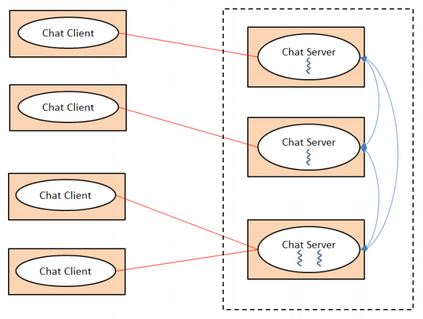
\includegraphics[scale=0.9]{strike_architecture.jpg}
\centering
\end{figure}

\subsection{Requirement Specification}
To begin with, we will discuss the requirement specification and assumption of the application logic. 

\begin{enumerate}[leftmargin=*]
\item Any chat client can connect to any chat server process to perform any of the following operations.

\item A chat client shall authenticate the user using username and password to let the user login to the system. This authenticated session shall maintain until the user logout from the system. The system should also invoke session timeout event to let the user auto-logout from the system if the user has been idle for a specified time. This authenticated session and all chat communication channel shall be encrypted and secured. 

\item An authenticated chat client shall let the user choose their prefer chat nickname (also known as identity or screen-name). After the user selected the nickname, this chat nickname shall be unique throughout the user current logon session. This nickname shall also be unique across all server processes i.e. if a user pick a chat nickname "victor" then no other user can create the same chat nickname until the user voluntarily logout or the session timeout has occurred.

\item Each server shall initially create the "MainHall" chat room suffix by server name e.g. if server name is 1 then it will have "MainHall-1" chat room. The logon user shall initially place into this "MainHall" chat room as a default chat room. Each server shall maintain a list of globally available chat rooms i.e. chat rooms from other server as well as chat rooms from locally connected clients. The connected clients shall be able to view this chat rooms list.

\item An authenticated chat client shall allow the user to create the chat room. A chat room will have a name and this chat room will be unique globally i.e. if a user creates a chat room name "joke" then no other user can create another chat room with the same name. Then the user who created the chat room shall become the owner for the chat room. A user can own one chat room at a time. If a client creates a chat room then that chat room will be managed by the server that the client is connected to.

\item An authenticated chat client shall allow the user to delete the chat room that they owned. Only the chat room owner shall be able to delete the chat room. The chat room owner shall delete the chat room first if he/she would like to join another chat room. A chat room is deleted if the owner client quits or disconnects abruptly. If the chat room is deleted, all users inside the chat room shall place into the default chat room i.e. "MainHall" of the connected server.

\item An authenticated chat client shall allow the user to join the chat room. Clients who are members of a chat room must be connected to the server managing that chat room. If a client joins a room managed by the server it is connected to then the server simply places the client in the corresponding room. If the room is managed by another server then the server sends a message to the client redirecting it to the server managing that chat room, without login again.

\item If a chat client disconnects abruptly or quit then the server should handle this and perform a graceful de-registering of the chat nickname and chat room (if owner) from the server. It should also notify this event to its all peer servers and all the peer servers should perform necessary measure to maintain each of their own server state.

\item The chat message must be forwarded to the connected server and, the server should broadcast this chat message to all clients inside the chat room that the user is sending to. The chat server should timestamp the chat message using UTC\footnote{Coordinated Universal Time} before broadcasting back to all the clients. The chat server should synchronize the system time with external NTP\footnote{Network Time Protocol} server in correct timezone.

\item If a chat server crashes or stops responding then other chat servers should detect this situation --- Failure Detection. All chatrooms on that server should be removed from the list and clients should not be redirected to that server anymore until it come back to alive. The connected clients are simply getting disconnected in the case of a chat server crash.

\end{enumerate}


\subsection{Protocol Design}
The core concept of Distributed Systems defines software components 
located at networked computers \textbf{communicate and coordinate their actions only by passing messages}\cite{coulouris}. The protocol specifies exactly how the clients-to-servers and server-to-server communication happen. Therefore, in our Strike System implementation, the protocol design becomes a crucial part of the system. The communication message has to be consistent and serializable. For this we choose JSON\footnote{http://www.json.org/} which is a lightweight data-interchangeable format. In the following example, it explains the basic building block of how JSON message are passing between client-server and server-server processes.

\begin{enumerate}[leftmargin=*]

\item Example: \textbf{List Server Protocol}
\\
The client can ask for the list of servers in the system and, send to server as a JSON message:
\begin{small}
\begin{verbatim}
{"type":"listserver"}
\end{verbatim}
\end{small}

The server replies with a list of all the servers in the system:
\begin{small}
\begin{verbatim}
{
    "type":"serverlist", "servers": 
    [ 
        {"serverid":"1", "address":"192.168.0.1", "port":"4444"}, 
        {"serverid":"2", "address":"192.168.0.2", "port":"4444"}
    ]
}
\end{verbatim}
\end{small}
In this example, the generated protocols are \verb|type|, \verb|listserver|, \verb|serverlist|, \verb|servers|, \verb|serverid|, \verb|address| and \verb|port|. This is a simple client-server protocol example. We will see a more moderate complex protocol example in next.

\item Example: \textbf{Login Authentication Protocol}
\\
At Login screen, the client send a user authentication message to the server:
\begin{small}
\begin{verbatim}
{"type":"authenticate", "username":"victor", "password":"cheese"}
\end{verbatim}
\end{small}
The chat server will then check the username and password in user database and attempt to authenticate the user. If the authentication has failed, the server will response to the client with the message:
\begin{small}
\begin{verbatim}
{"type":"authresponse", "success":"false", "reason":"UnknownAccountException"}
\end{verbatim}
\end{small}
The user database can be a centralized database system such as making use of third party database management software. In our implementation, we use Apache Shiro\footnote{https://shiro.apache.org/} framework to make an abstraction for the concrete implementation. As such, the fail reason depends on this middleware specific exceptions. For example, \textit{UnknownAccountException}, \textit{IncorrectCredentialsException}, \textit{LockedAccountException}, \textit{AuthenticationException} are possible Shiro exceptions that can response to the client.
However, if the authentication is success, the chat server response to the client with message:
\begin{small}
\begin{verbatim}
{"type":"authresponse", "success":"true", "reason":"none"}
\end{verbatim}
\end{small}
And the chat server also send to all other servers with message:
\begin{small}
\begin{verbatim}
{
    "type":"notifyusersession", "sessionid":"ba64077b-85b4-40f0-a5ac-480ad3e341b3", 
    "username":"victor", "serverid":"1", "status":"login"
}
\end{verbatim}
\end{small}
And if the user logout, the chat server send to all other servers with message:
\begin{small}
\begin{verbatim}
{
    "type":"notifyusersession", "sessionid":"ba64077b-85b4-40f0-a5ac-480ad3e341b3",
    "username":"victor", "serverid":"1", "status":"logout"
}
\end{verbatim}
\end{small}




\end{enumerate}






\subsection{Complete Design}

However, a more complete system architecture of Strike production system can be illustrated as in Figure~\ref{fig:strike_arch_comp}. 

\begin{figure}[h]
\caption{Strike Architecture Production}
\label{fig:strike_arch_comp}
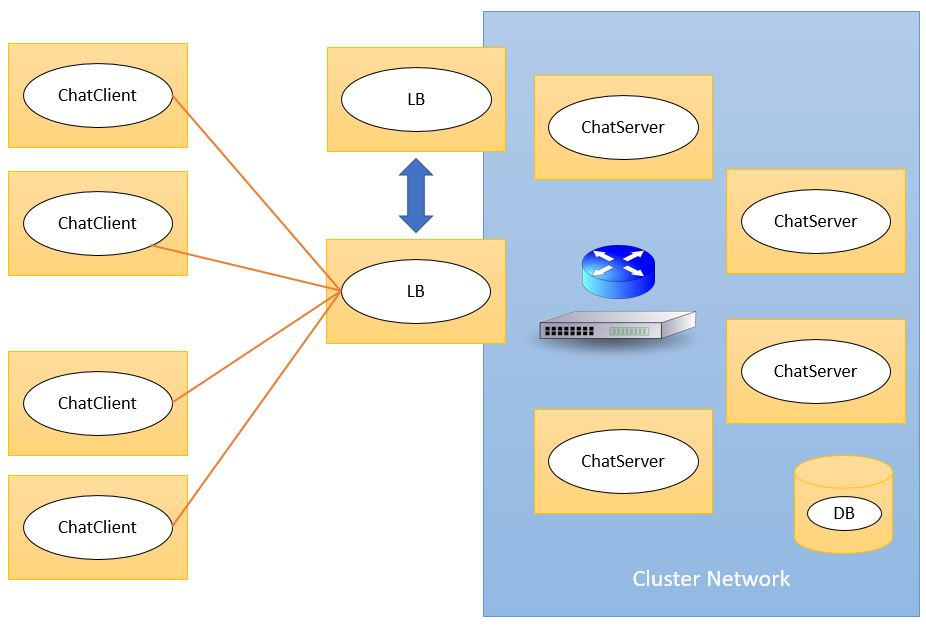
\includegraphics[scale=0.6]{strike_architecture_prod.jpg}
\centering
\end{figure}


\end{document}